%----------------------------------------------------------------------------------------
%
% LaTeX-template for degree projects at LNU, Department of Computer Science
% Last updated by Johan Hagelbäck, Oct 2015
% Linnaeus University
%
% License: Creative Commons BY
%
%----------------------------------------------------------------------------------------

%----------------------------------------------------------------------------------------
%	Settings and configuration
%----------------------------------------------------------------------------------------

\documentclass[a4paper,12pt]{article}
\usepackage[T1]{fontenc}
\usepackage{times}
\usepackage[english]{babel}
\usepackage[utf8]{inputenc}
\usepackage{caption}
\usepackage{subcaption}
\usepackage{wallpaper}
\usepackage[absolute]{textpos}
\usepackage[top=2cm, bottom=2.5cm, left=3cm, right=3cm]{geometry}
\usepackage{appendix}
\usepackage[nottoc]{tocbibind}
\usepackage[hidelinks]{hyperref}
\setcounter{figure}{0}
%\setcounter{secnumdepth}{3}
%\setcounter{tocdepth}{3}
\usepackage{amsmath}
\numberwithin{figure}{section}
\usepackage{sectsty}
\sectionfont{\fontsize{14}{15}\selectfont}
\subsectionfont{\fontsize{12}{15}\selectfont}
\subsubsectionfont{\fontsize{12}{15}\selectfont}

\usepackage{csquotes} % Used to handle citations

\renewcommand{\thetable}{\arabic{section}.\arabic{table}}  
\renewcommand{\thefigure}{\arabic{section}.\arabic{figure}} 

%----------------------------------------------------------------------------------------
%	
%----------------------------------------------------------------------------------------
\newsavebox{\mybox}
\newlength{\mydepth}
\newlength{\myheight}

\newenvironment{sidebar}%
{\begin{lrbox}{\mybox}\begin{minipage}{\textwidth}}%
{\end{minipage}\end{lrbox}%
 \settodepth{\mydepth}{\usebox{\mybox}}%
 \settoheight{\myheight}{\usebox{\mybox}}%
 \addtolength{\myheight}{\mydepth}%
 \noindent\makebox[0pt]{\hspace{-20pt}\rule[-\mydepth]{1pt}{\myheight}}%
 \usebox{\mybox}}

%----------------------------------------------------------------------------------------
%	Title section
%----------------------------------------------------------------------------------------
\newcommand\BackgroundPic{
    \put(-2,-3){
    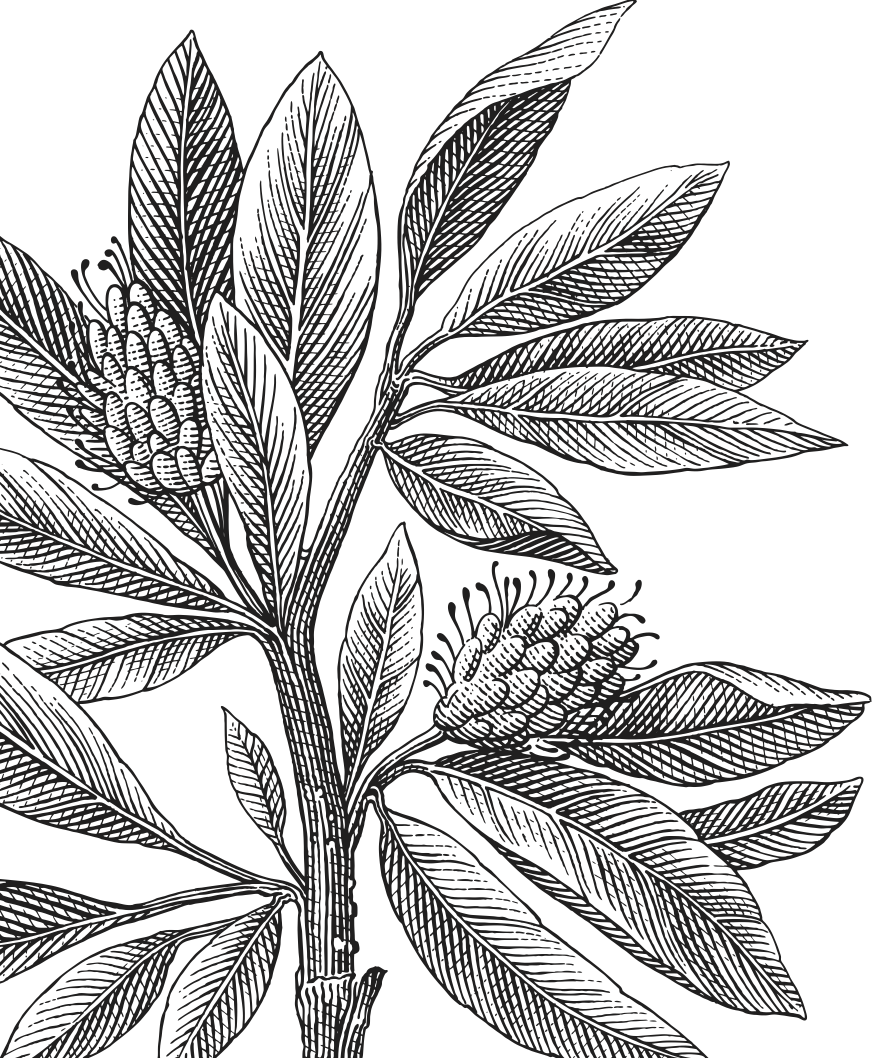
\includegraphics[keepaspectratio,scale=0.3]{img/lnu_etch.png} % Background picture
    }
}
\newcommand\BackgroundPicLogo{
    \put(30,740){
    
\includegraphics[keepaspectratio,scale=0.10]{img/logo.png} % Logo in upper left corner
    }
}

\title{	
\vspace{-8cm}
\begin{sidebar}
    \vspace{10cm}
    \normalfont \normalsize
    %\Huge Bachelor/Master Thesis Project \\
    \vspace{-1.3cm}
\end{sidebar}
\vspace{3cm}
\begin{flushleft}
    \huge Computer networks - 1DV701 \\ 
    \LARGE  Assignment 2\\
\end{flushleft}
\null
\vfill
\begin{textblock}{6}(10,13)
\begin{flushright}
\begin{minipage}{\textwidth}
\begin{flushleft} \large
\emph{Author:} Michael Johansson \& Jakob Heyder\\ % Author
%\emph{Supervisor:} Name of your supervisor\\ % Supervisor
%\emph{Examiner:} Dr.~Mark \textsc{Brown}\\ % Examiner (course manager)
\emph{Semester:} VT 2017\\ % 
%\emph{Subject:} Computer Science\\ % Subject area
\end{flushleft}
\end{minipage}
\end{flushright}
\end{textblock}
}

\date{} 

\begin{document}
\pagenumbering{gobble}
\newgeometry{left=5cm}
\AddToShipoutPicture*{\BackgroundPic}
\AddToShipoutPicture*{\BackgroundPicLogo}
\maketitle
\restoregeometry
\clearpage


%----------------------------------------------------------------------------------------
\newpage
\pagenumbering{gobble}
\tableofcontents % Table of contents
\newpage
\pagenumbering{arabic}

%----------------------------------------------------------------------------------------
%
%	Here follows the actual text contents of the report.
%
%----------------------------------------------------------------------------------------

\section{Assignment summary}

\begin{itemize}
\item\textbf{Michael} did the most of the report and implemented exceptions handling. Wrote some methods in the code and did tests.

Work percentage 45\%

\item\textbf{Jakob} did most of the server code, with the major parts of the functionality. He did the Javascript pages for PUT/POST. He also made sure that we had a good ground to stand on with alot of enumeration types for MIME types etc.

Work percentage 55\%
\end{itemize}

\subsection{Small summary of our server}

It all starts with that we have our class HTTPReader that reads and parse the the request and then return a HTTPRequest object. 

This HTTPRequest we use in our HTTPResponseFactory class that is the heart of our server where we take the request and build our response from that. So in our factory we check if the request was a GET, POST or PUT and respond accordantly.

When the factory then is done building the response we write it out to the outputStream as an byte array stream. 

If there is any error we throw an exception and from that exception create different responses that we send to the client. 


\subsection{Good to know}
\begin{itemize}
	\item We have an out commented code where we can test our HTTP version not implemented exception. 
	
	\item We choose to close the connection after each request/response but we could alternatively left it open and let the server time out the connection
	
	\item Only GET,POST and PUT are implemented HTTP metods.
	
	\item Our POST/PUT gives Unsupported Media type for uploading something that is not in our MIME types.
	
	\item ../ and any URI with secret are restricted and will give 403.
	
	\item Due to the human readability issues of the hash-function generated filenames in our PUT/POST, we display a list of all images in the /images/ folder when trying to PUT an image, so if the client want to update an image he can look up his hash for the image and from that update that file.
\end{itemize}

\newpage

\section{Problem one}

We choose to create an Index file every time an user requests a directory. This way we have index links to the files in that directory to help with the navigation and it looks good. But if the user ask for a file/directory that doesn't exist on the server we send back a 404(File not found).We also link to our secret folder in this main index but if we click on it we get an 403 (access denied).
 
\begin{figure}[h!]
	\centering
	\label{Directory}
	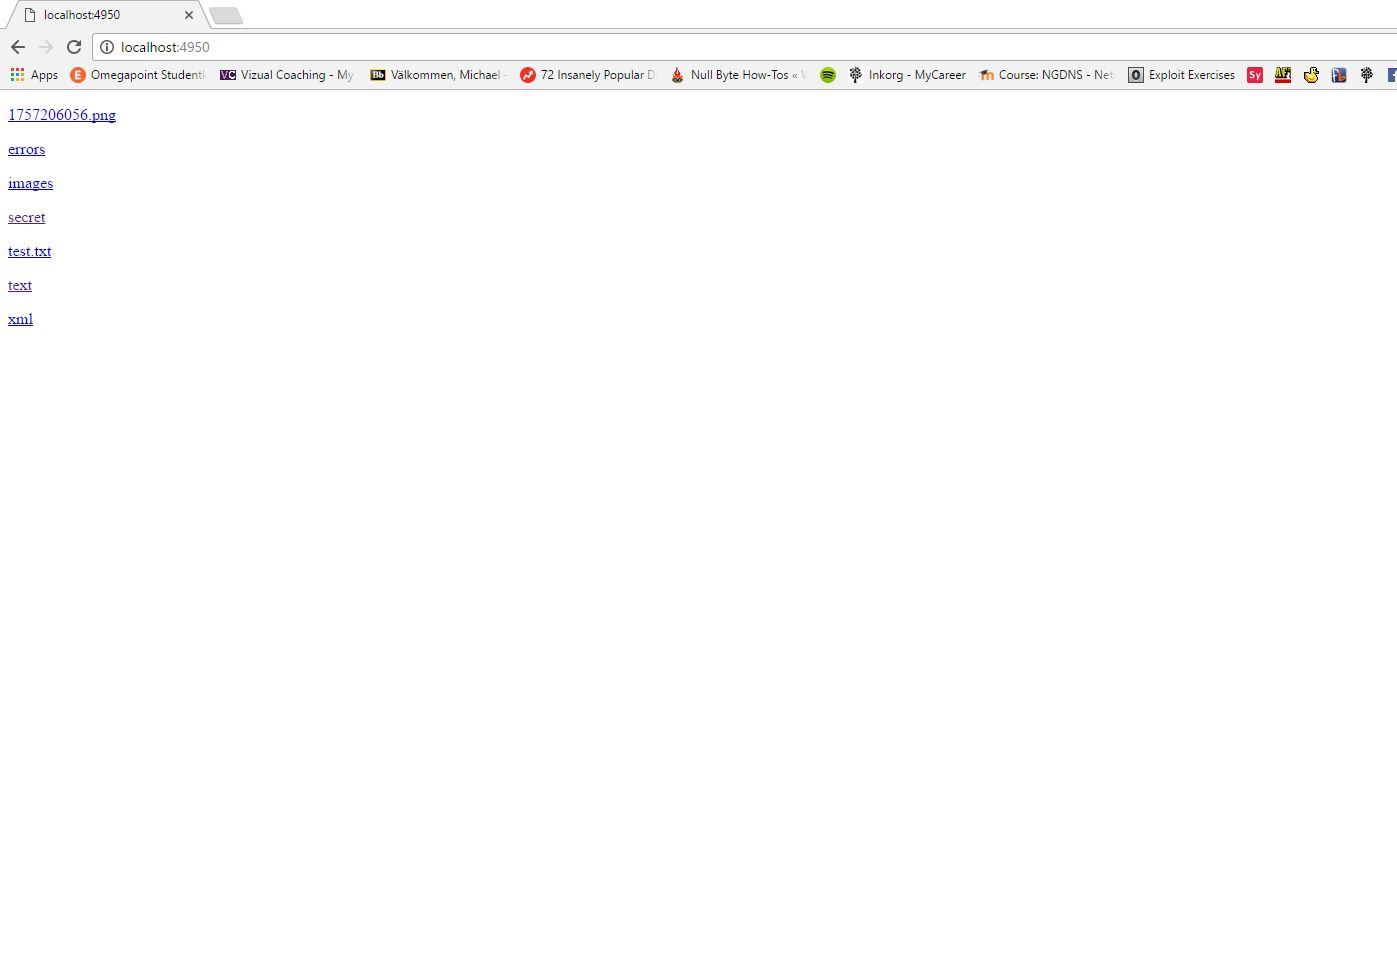
\includegraphics[width=0.95\textwidth,keepaspectratio]{img/Directory.jpg} 
	\caption{GET request on a directory, responds with index.html}
\end{figure}

\begin{figure}[hp!]
	\centering
	\label{HTML}
	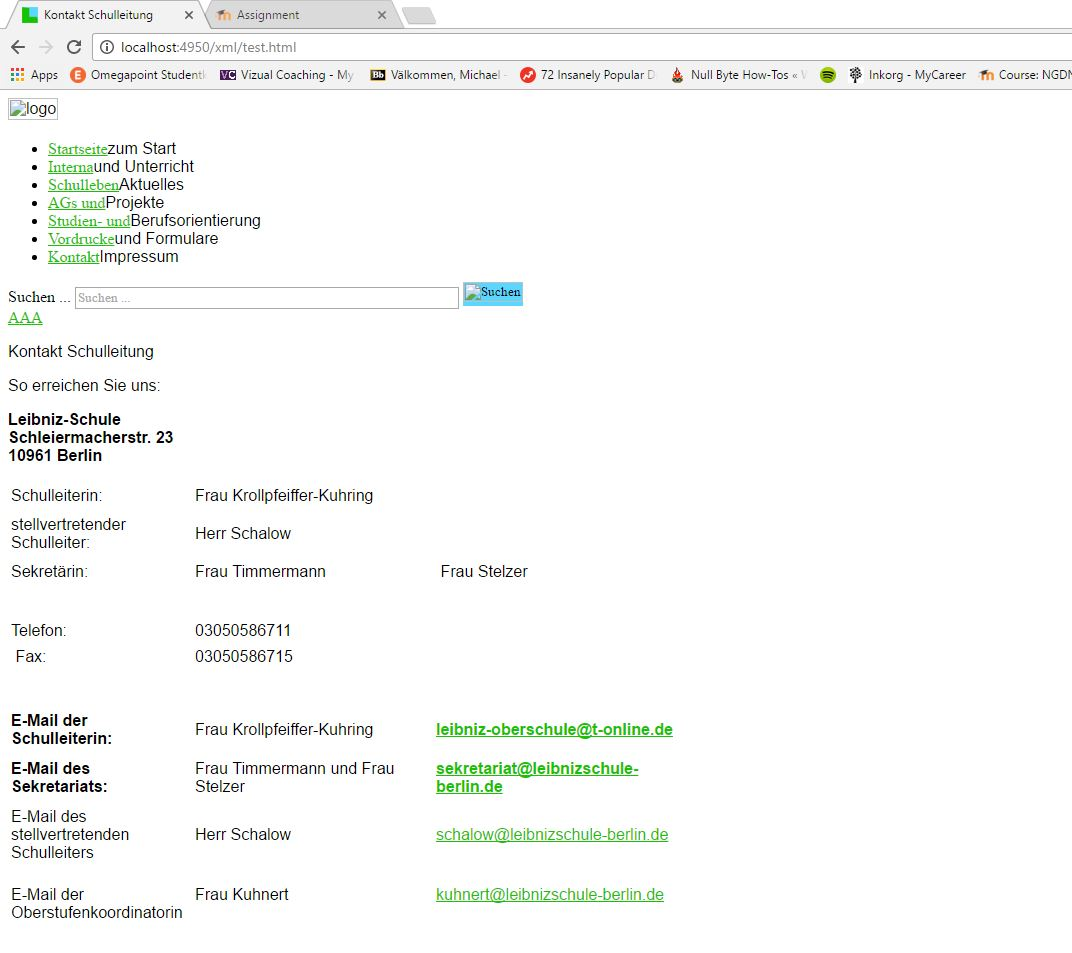
\includegraphics[width=0.95\textwidth,keepaspectratio]{img/HTMLFile.jpg} 
	\caption{GET request on a HTML file, this one is a copy without css of a German site}
\end{figure}

\begin{figure}[hp!]
	\centering
	\label{PNG}
	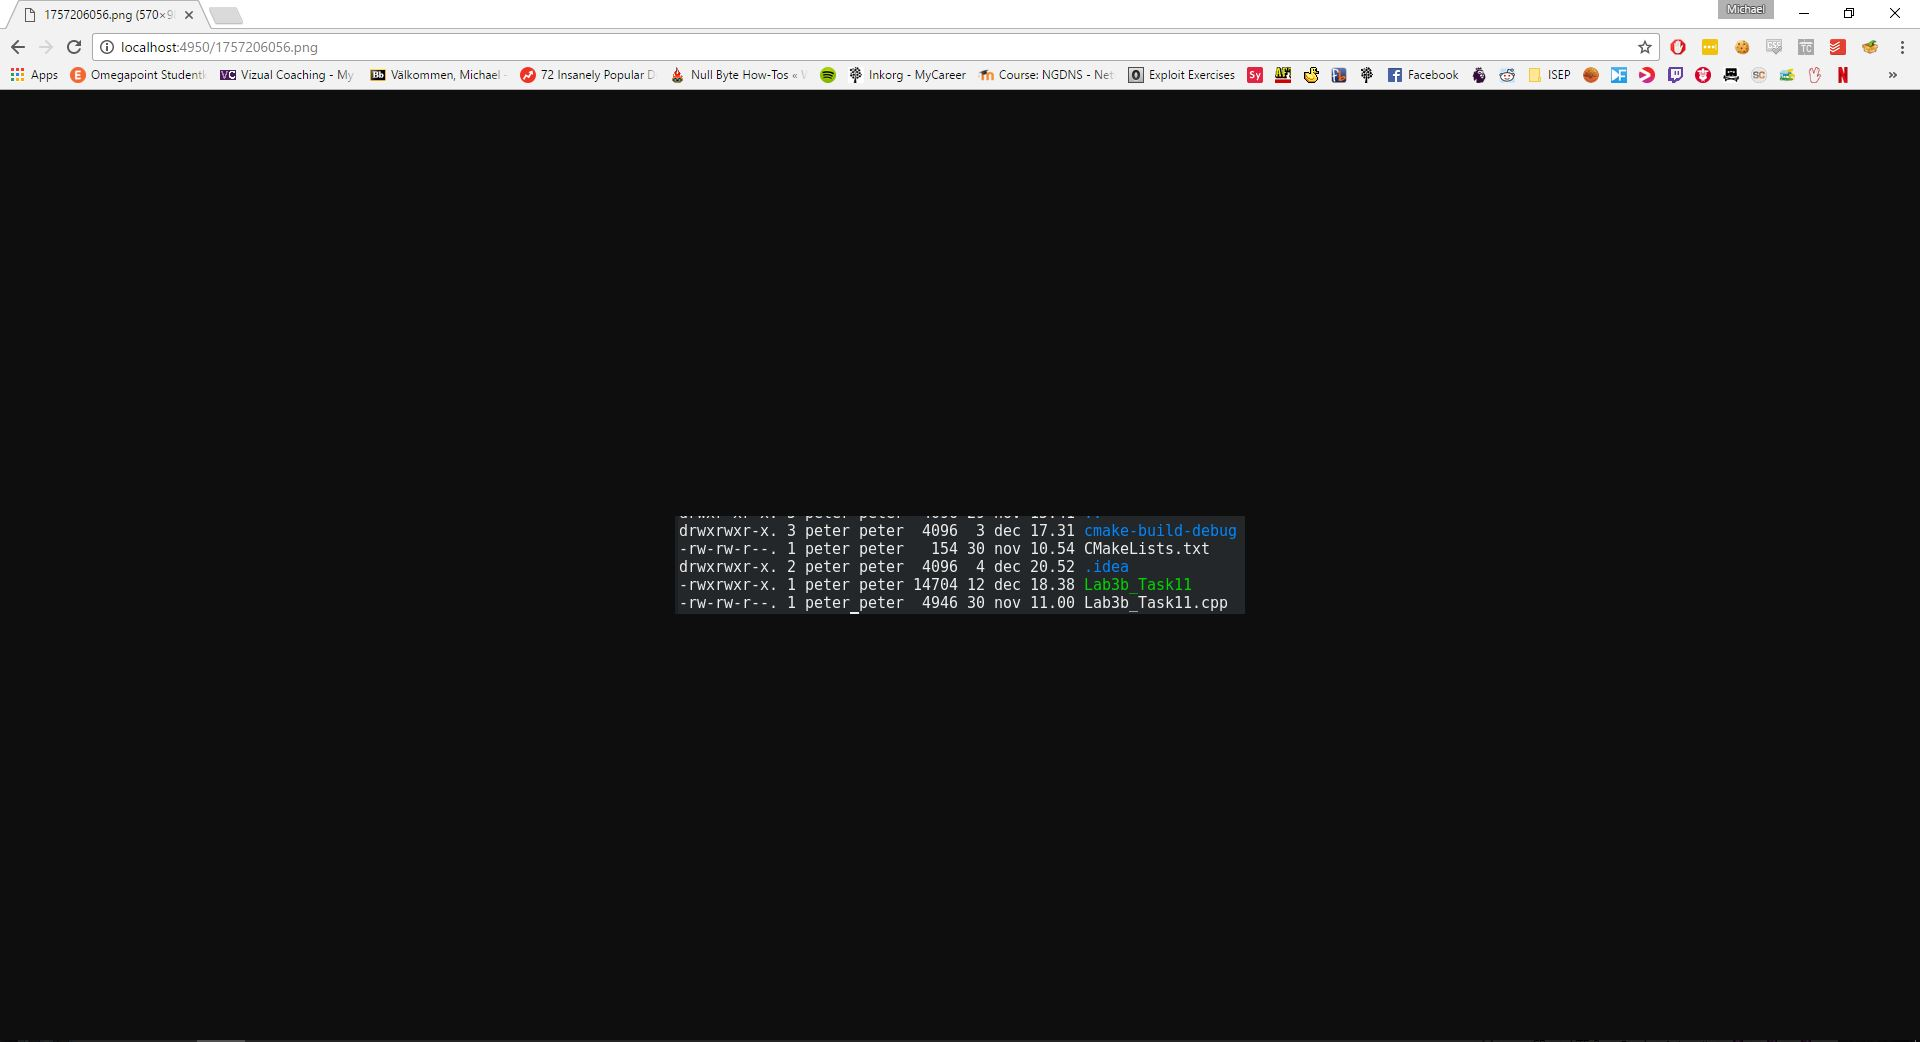
\includegraphics[width=0.95\textwidth,keepaspectratio]{img/PNGFile.jpg} 
	\caption{GET request on an image}
\end{figure}

\newpage
\section{Problem two}

List of all implemented server responses
\begin{itemize}
	\item 200: OK
	\item 201: Created
	\item 204: No Content
	\item 302: Found
	\item 400: Bad request
	\item 403: Access Denied
	\item 404: Not Found
	\item 411: Length Required
	\item 414: URI Too Long
	\item 415: Unsupported Media Type
	\item 500: Internal Server Error
	\item 501: Not implemented
	\item 505: HTTP Version Not Supported
\end{itemize}

\begin{figure}[h!]
	\centering
	\label{Access denied}
	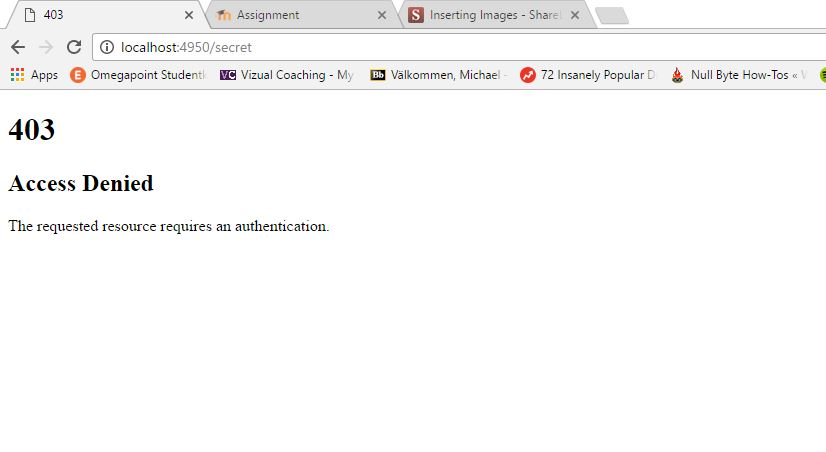
\includegraphics[width=0.90\textwidth,keepaspectratio]{img/403.jpg} 
	\caption{403 Access denied when trying to access our secret folder}
\end{figure}

\begin{figure}[h!]
	\centering
	\label{not found}
	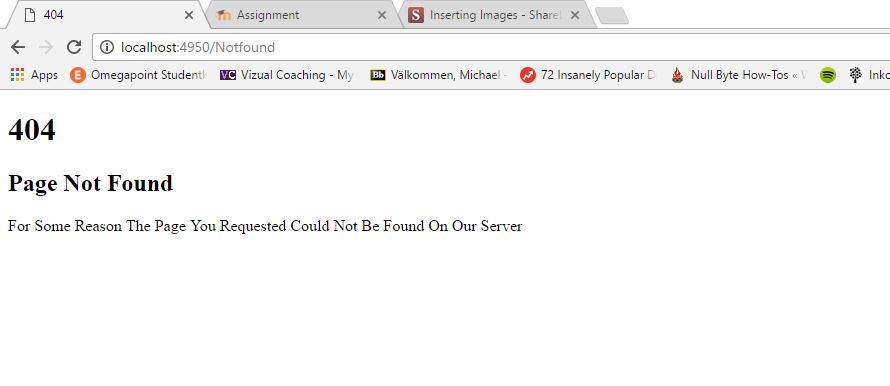
\includegraphics[width=0.90\textwidth,keepaspectratio]{img/404.jpg} 
	\caption{404 Not Found when trying to GET a resource that don't exist on the server}
\end{figure}

\begin{figure}[h!]
	\centering
	\label{Server error}
	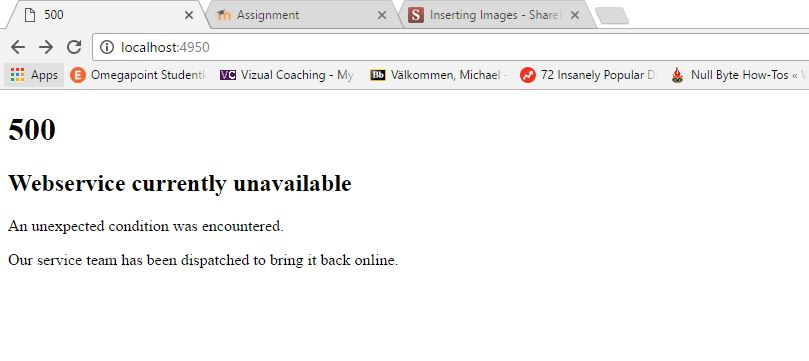
\includegraphics[width=0.90\textwidth,keepaspectratio]{img/500.jpg} 
	\caption{500 for any internal server errors, socket error etc.}
\end{figure}

\newpage
\subsection{VG.1 HTTP status code implementation}

For some images below we just show the error.html response but we send the status code as well for every error.

\begin{figure}[h!]
	\centering
	\label{201}
	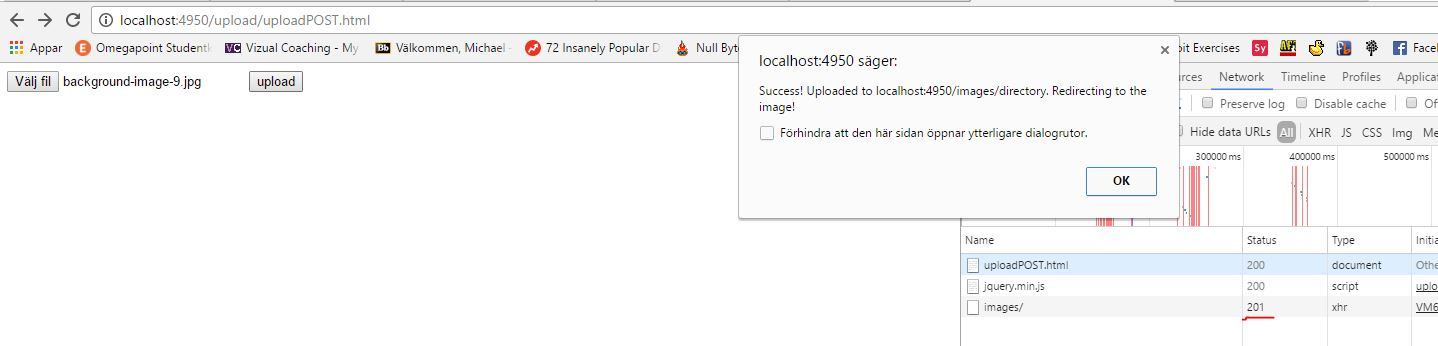
\includegraphics[width=0.95\textwidth,keepaspectratio]{img/201.jpg} 
	\caption{201 Created, when the user creates a new resource with POST/PUT.}
\end{figure}

\begin{figure}[h!]
	\centering
	\label{204}
	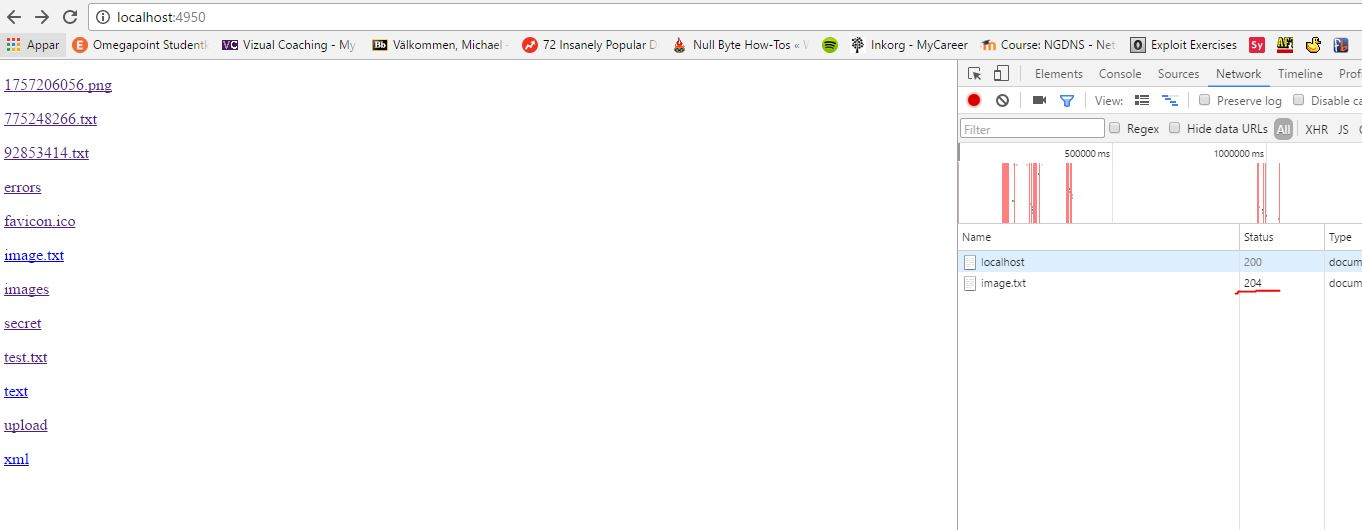
\includegraphics[width=0.95\textwidth,keepaspectratio]{img/204.jpg} 
	\caption{204 Not Found, if the user tries to GET a empty file}
\end{figure}

\begin{figure}[h!]
	\centering
	\label{302}
	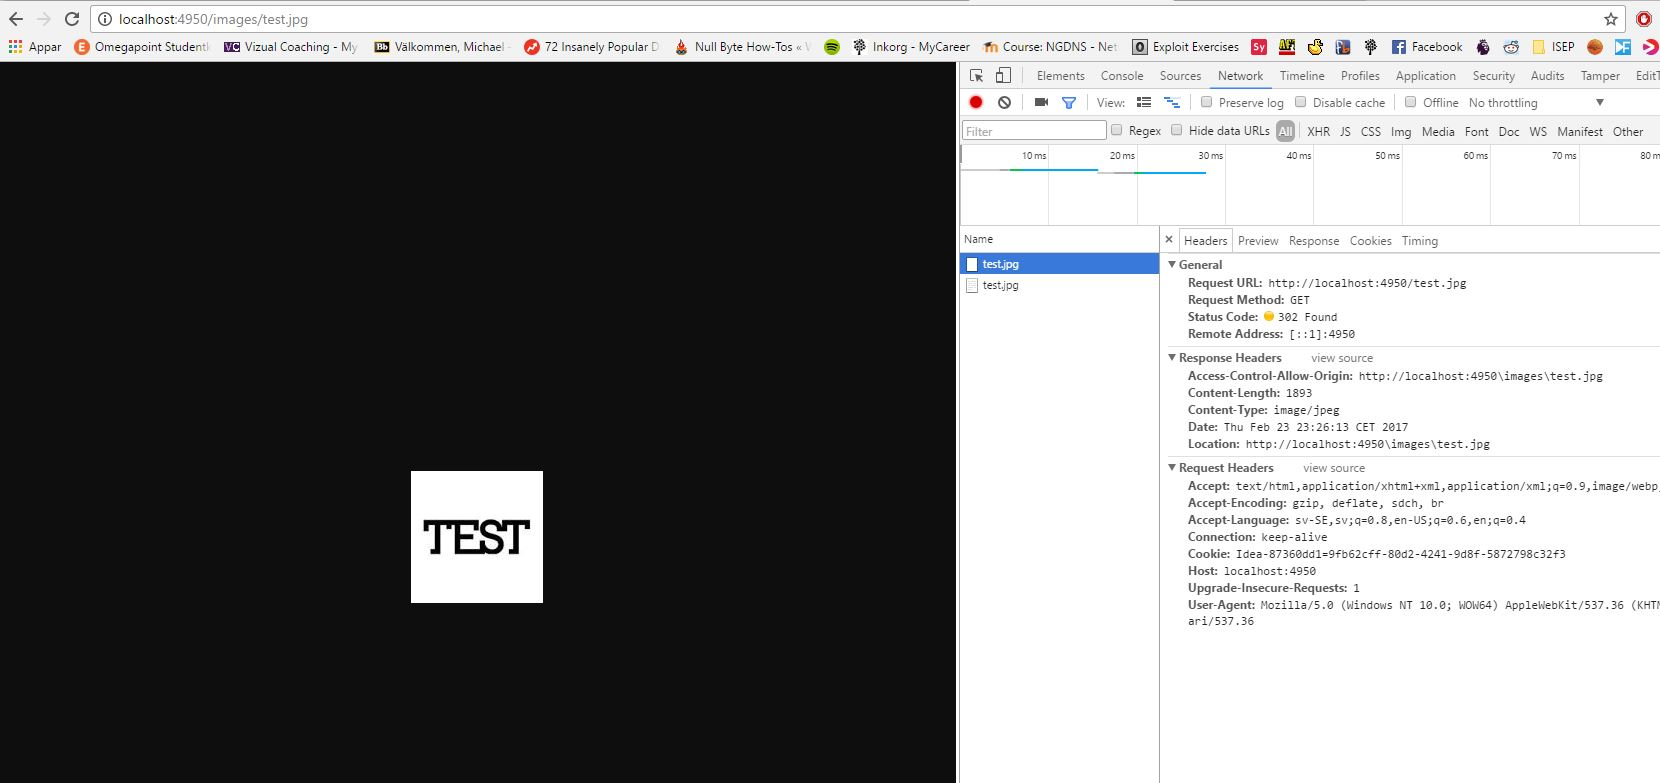
\includegraphics[width=0.95\textwidth,keepaspectratio]{img/302.jpg} 
	\caption{302 if we have specified that a specific file has changed location on the server, redirect the browser to the new location with the location header.}
\end{figure}

\begin{figure}[h!]
	\centering
	\label{400}
	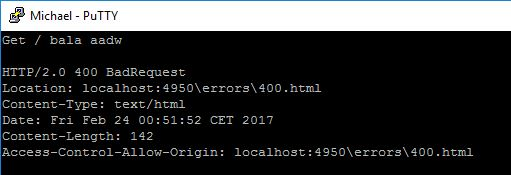
\includegraphics[width=0.95\textwidth,keepaspectratio]{img/400.jpg} 
	\caption{400 if request has malformed syntax}
\end{figure}

\begin{figure}[h!]
	\centering
	\label{411}
	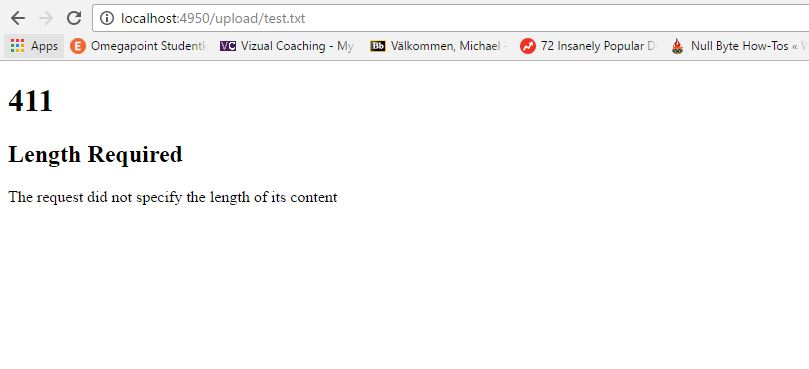
\includegraphics[width=0.95\textwidth,keepaspectratio]{img/411.jpg} 
	\caption{411 if the POST/PUT body is empty}
\end{figure}

\begin{figure}[h!]
	\centering
	\label{414}
	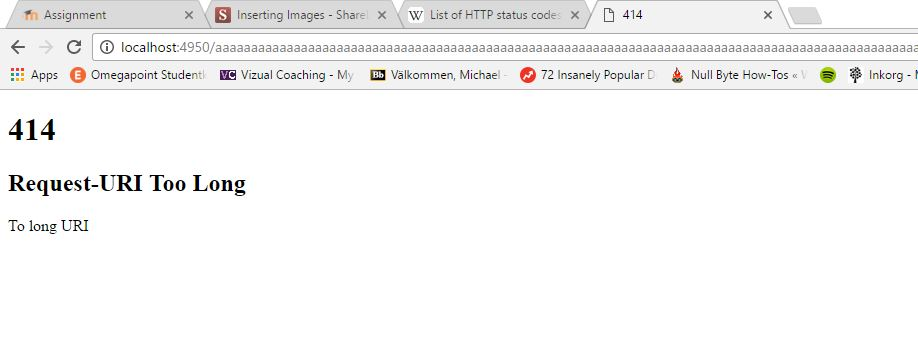
\includegraphics[width=0.95\textwidth,keepaspectratio]{img/414.jpg} 
	\caption{414 if the URI is longer then 2048 characters.}
\end{figure}

\begin{figure}[h!]
	\centering
	\label{415}
	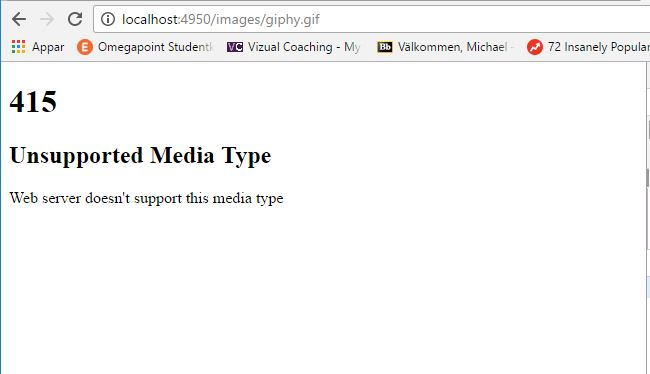
\includegraphics[width=0.95\textwidth,keepaspectratio]{img/415.jpg} 
	\caption{415 we get this when the client tries to POST/PUT a exe/docx etc.}
\end{figure}

\begin{figure}[h!]
	\centering
	\label{501}
	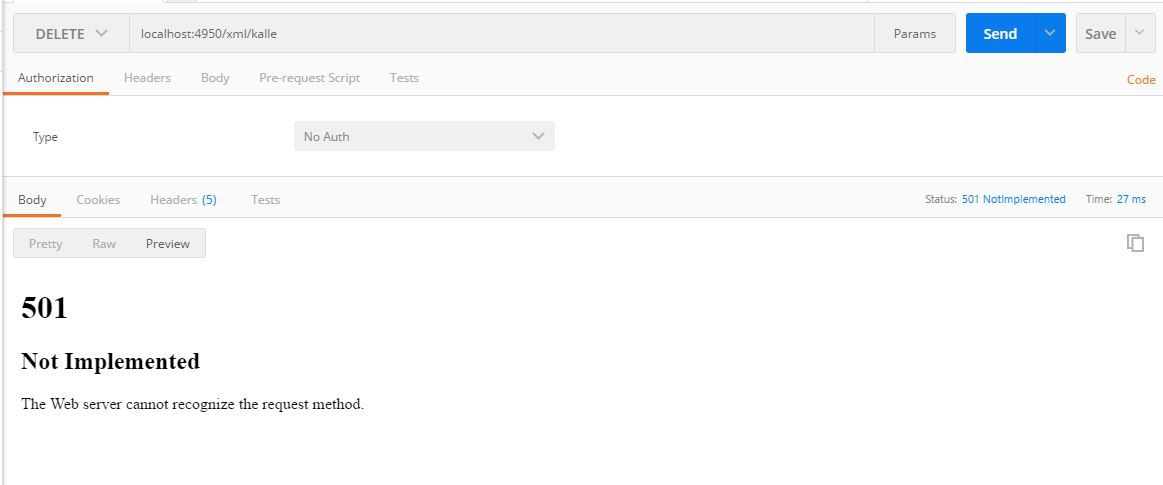
\includegraphics[width=0.95\textwidth,keepaspectratio]{img/501.jpg} 
	\caption{501 for any HTTP methods that we haven't implemented, like in this case the DELETE method.}
\end{figure}

\begin{figure}[h!]
	\centering
	\label{505}
	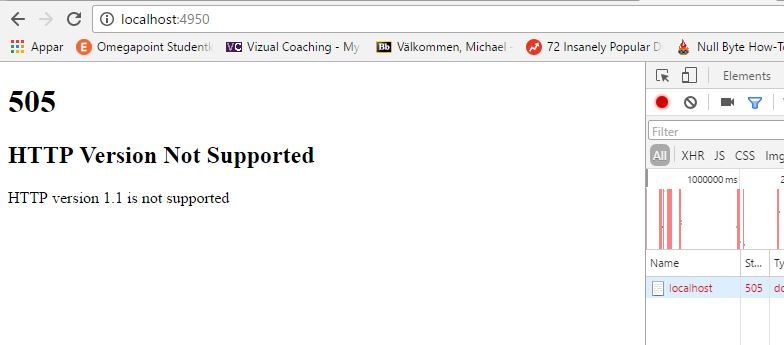
\includegraphics[width=0.95\textwidth,keepaspectratio]{img/505.jpg} 
	\caption{505 for HTTP version 1.1. We support all HTTP versions when we run the server, but we can set this exception if we don't want to support a special HTTP version later on.}
\end{figure}

\newpage
\subsection{VG.2 POST vs PUT}

We use POST when the user uploads a new resource that our sever handles where it should be placed. In our POST implementation the user can upload an image through our upload page. The server then creates that images with a hash as the file name and under the images folder.  

If instead the user has the exact request-URI then we can use PUT to create or overwrite the file on that exact URI. 

So in short the POST is used for when the client don't need to know the exact URI and just upload the file where we want it. The PUT when the client want to Create or replace a file on an exact URI.

\newpage

\section{Problem three}

Using Telnet we are creating a raw TCP connection that sends and receive plain text. So as we se in figure \ref{TEXT} for our request for a text file we get the text as is. But if we then ask for an image like in figure \ref{IMAGE} we get the image information as text as well. So the Telnet interprets the image binary as plain text and that's why we get those weird symbols.

\begin{figure}[h!]
	\centering
	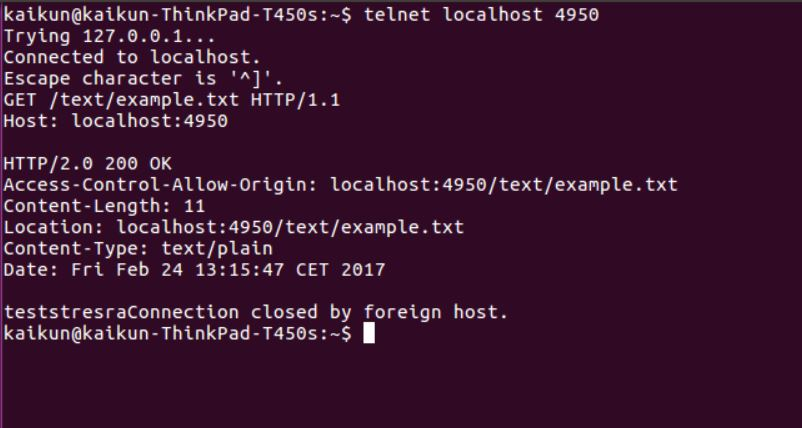
\includegraphics[width=0.95\textwidth,keepaspectratio]{img/TEXT.jpg} 
	\caption{Telnet client asking for a .txt file, reads it in plain text}
	\label{TEXT}
\end{figure}

\begin{figure}[h!]
	\centering
	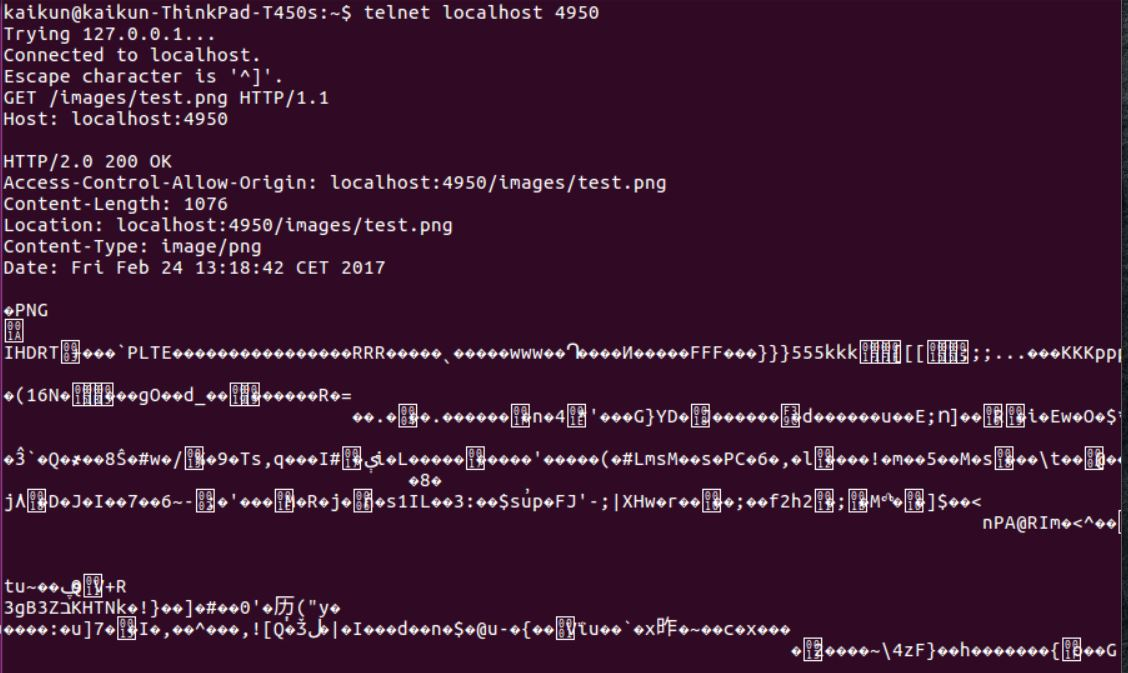
\includegraphics[width=0.95\textwidth,keepaspectratio]{img/IMAGE.jpg} 
	\caption{Telnet client asking for a .PNG file, also reads it as plain text}
	\label{IMAGE}
\end{figure}

\end{document}
